\section{Auswertung}
\label{sec:Auswertung}
Alle im Folgenden berechneten Ergebnisse sind wegen dieser Fehlerbehaftungen $\mathup{\Delta}x_\text{i}$ mit Abweichungen nach dem \textsc{Gauss}schen Theorem der Fehlerfortpflanzung angegeben \cite{uncertainties}. Für die Gesamtabweichung $\mathup{\Delta}f$ einer berechneten Größe gilt

\begin{equation}
	\mathup{\Delta}f(x_1,...,x_\text{N})=\sqrt{\sum_{\text{i}=1}^\text{N}\left(\frac{\partial f}{\partial x_\text{i}}\mathup{\Delta}x_\text{i}\right)^2}.
	\label{eq:gauss_gen}
\end{equation}
\newpage
\subsection{Abstimmen der Systemparameter}
\begin{figure}
	\centering
	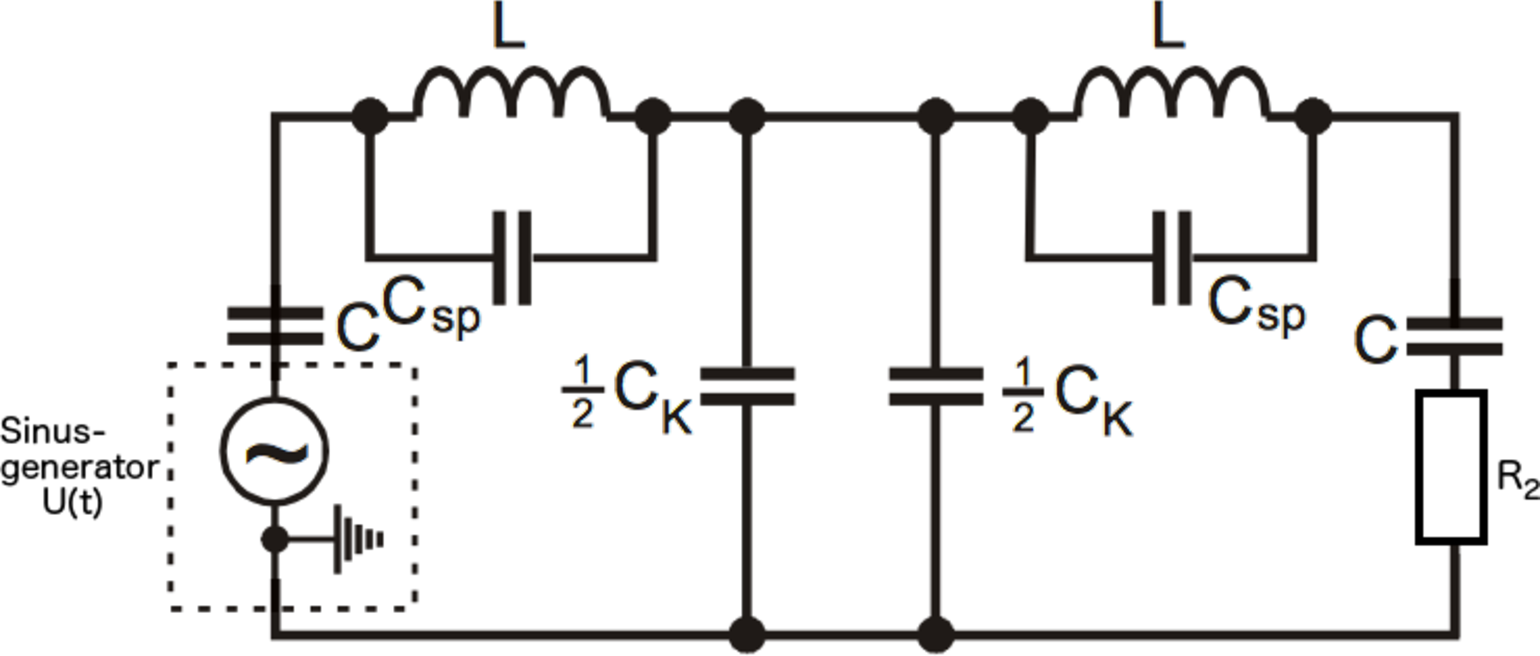
\includegraphics[width=0.5\textwidth]{Bilder/Auswertungsaufbau.pdf}
	\caption{Ersatzschaltung für die Auswertung. \cite{v355} \cite{gimp}}
	\label{fig:ersatz}
\end{figure}
\begin{table}[ht]
	\centering
	\begin{tabular}{ccc}
	\toprule
	{Kapazität $C$}&{Kapazität der Spule $C_\mathup{sp}$}&{Induktivität der Spule $L$}\\
	{$[\si{\pico\farad}]$}&{$[\si{\pico\farad}]$}&{$[\si{\milli\henry}]$}\\
	\midrule
		798\pm2 &37\pm1 &31.90\pm0.05\\
	\bottomrule
	\end{tabular}
	\caption{Die festen Parameter des gekoppelten Systems nach Abbildung \ref{fig:ersatz}. \cite{v355}}
\end{table}
Der Kopplungskondensator $C_\mathup{K}$ wird überbrückt und somit effektiv nur der linke Schwingkreis angeregt.
%Die Frequenz des Generators, bei welchem die Widerstandsspannung $U_\mathup{R_1}(t)$ maximal wird, ist die Resonanzfrequenz $f_\text{Res}$ des Systems. 
Die Resonanzfrequenz $f_\text{Res}$ des Systems wurde mit $f_\text{Res} = \SI{30.74}{\kilo\hertz}$ bei maximaler Widerstandsspannung $U_\mathup{R_1}(t)$
grob abgeschätzt.\\
Der Phasenwinkel $\phi$ zwischen Erregerspannung $U(t)$ und der Widerstandsspannung $U_\mathup{R_1}(t)$ ist gleich Null, sofern die Erregerspannung $U(t)$ die Resonanzfrequenz $f_\text{Res}$ aufweist.
%Beim Auftragen der Widerstandsspannung $U_\mathup{R_1}(t)$ gegen die Erregerspannung $U(t)$ wird eine Lissajous-Figur sichtbar.
%Für den Phasenwinkel $\phi=0$ ist die Lissajous-Figur nicht-elliptisch, gerade und verläuft im ersten und dritten Quadranten des Oszilloskopes.
Die Resonanzfrequenz $f_\text{Res}$ wird mithilfe des in Abschnitt \ref{sec:Resonanzfrequenz} beschriebenen Verfahrens auf den Wert
\begin{equation}
	f_\text{Res} = \SI{30.71}{\kilo\hertz}
\end{equation} präzisiert.
Der %aus Abschnitt \ref{sec:Theorie} 
für gedämpfte Schwingkreise bekannte Erwartungswert \cite{v354} für die Resonanzfrequenz ist
\begin{alignat}{2}
	f_\text{Res, Theorie} = \sqrt{\frac{1}{\mathup{LC_\text{Gesamt}}}-\frac{\mathup{R^2}}{4\mathup{L^2}}} = \SI{30.84\pm0.05}{\kilo\hertz}, &\quad\mathup{\Delta}f_\text{Res}=-0,42\,\%
	\label{eq:fres12}
\end{alignat}
In der Theorie werden ideale Komponenten angenommen.
Zur Berücksichtigung, dass eine reale Spule eine nicht zu vernachlässigende Induktivität $C_\text{sp}$ aufweist, werden für die Auswertung im Allgemeinen angepasste Gesamtkapazitäten betrachtet. Für \eqref{eq:fres12} gilt daher $C_\text{Gesamt}= C+C_\text{sp}$

Der zweite Schwingkreis wird durch seinen variablen Kondensator $C$ mithilfe einer \textsc{Lissajous}-Figur an den ersten Schwingkreis angeglichen.
\subsection{Untersuchung der Schwebung}
\label{sec:Auswertung1}
\begin{table}[h!]
	\centering
	\begin{tabular}{cccc}
	\toprule
	{Kopplungskapazität}&\multicolumn{3}{c}{Frequenzverhältnis}\\
	{$C_\mathup{K}$}&{$\alpha$}&{$\alpha_\text{Theorie}$}&{$\mathup{\Delta}\alpha$}\\
	{$[\si{\nano\farad}]$}&{[1]}&{[1]}&{[1]}\\
	\midrule
		$\SI{9.99(9)}{}$& 14&	14.2\pm0.14		&-0.2\\
		$\SI{8.00(8)}{}$& 11&	11.6\pm0.11		&-0.6\\
		$\SI{6.47(6)}{}$&  9&	9.6\pm0.09 		&-0.6\\
		$\SI{5.02(5)}{}$&  7&	7.6\pm0.07 		&-0.6\\
		$\SI{4.00(4)}{}$&  6&	6.3\pm0.06 		&-0.3\\
		$\SI{3.00(3)}{}$&  5&	5.0\pm0.04 		&-0.0\\
		$\SI{2.03(2)}{}$&  4&	3.7\pm0.03 		& 0.3\\
		$\SI{1.01(1)}{}$&  2&	2.3\pm0.02 		&-0.3\\
	\bottomrule
	\end{tabular}
	\caption{Die Frequenzverhältnisse $\alpha$ in Abhängigkeit von der Kopplungskapazität $C_\mathup{K}$.}
	\label{tab:verhaeltnis}
\end{table}
Die Widerstandsspannung $U_\mathup{R_2}(t)$ ist ein Maß für den Strom $I_\mathup{2}(t)$, es besteht nach Ohmschen Gesetz der Zusammenhang $U(t)=\mathup{R}\cdot I(t)$ bei konstantem Widerstand R.
Bei dem Auftragen der Widerstandsspannung $U_\mathup{R_2}(t)$ gegen die Zeit wird wie in Abbildung \ref{fig:schwebung} eine Schwebung sichtbar.
Um das Verhältnis der Schwebungs- und Schwingungsfrequenz zu bestimmen, wird innerhalb einer Schwebungsperiode die Anzahl der Schwingungsmaxima abgezählt, der Erwartungswert ist aus Abschnitt \ref{sec:Theorie} gegeben. 
Es gilt
\begin{alignat}{3}
	\alpha=\frac{n_\text{Max.Osz.}}{n_\text{Max.Schweb.}} &\quad\text{und} &&\quad\alpha_\text{Theorie}=\frac{f_++f_−}{2(f_+−f_−)},
\end{alignat}
es ergibt sich die Tabelle \ref{tab:verhaeltnis}.
\subsection{Untersuchung der Fundamentalfrequenzen}
\label{sec:Auswertung2}
\begin{table}[h!]
	\centering
	\begin{tabular}{ccccccc}
	\toprule
	{Kopplungskapazität}&\multicolumn{4}{c}{Fundamentalfrequenz}&\multicolumn{2}{c}{Abweichung}\\
	{$C_\mathup{K}$}&{$f_\mathup{+}$}&{$f_\mathup{-}$}&{$f_\mathup{+,Theorie}$}&{$f_\mathup{-,Theorie}$}&$\mathup{\Delta}f_\mathup{+}$&$\mathup{\Delta}f_\mathup{+}$\\
	{$[\si{\nano\farad}]$}&{$[\si{\kilo\hertz}]$}&{$[\si{\kilo\hertz}]$}&{$[\si{\kilo\hertz}]$}&{$[\si{\kilo\hertz}]$}&{$[\%]$}&{$[\%]$}\\
	\midrule
		$\SI{9.99(9)}{}$	&30.56	&32.85	 &30.84\pm0.05	&33.09\pm0.05 	&0.90 	&0.73\\
		$\SI{8.00(8)}{}$	&30.57	&33.38	 &30.84\pm0.05	&33.63\pm0.06 	&0.87 	&0.73\\
		$\SI{6.47(6)}{}$	&30.57	&33.98	 &30.84\pm0.05	&34.25\pm0.06 	&0.87 	&0.77\\
		$\SI{5.02(5)}{}$	&30.57	&34.88	 &30.84\pm0.05	&35.16\pm0.06 	&0.87 	&0.78\\
		$\SI{4.00(4)}{}$	&30.57	&35.86	 &30.84\pm0.05	&36.16\pm0.07 	&0.87 	&0.82\\
		$\SI{3.00(3)}{}$	&30.57	&37.40	 &30.84\pm0.05	&37.73\pm0.08 	&0.87 	&0.87\\
		$\SI{2.03(2)}{}$	&30.58	&40.12	 &30.84\pm0.05	&40.5 \pm0.1	&0.84 	&0.97\\
		$\SI{1.01(1)}{}$	&30.58	&47.23	 &30.84\pm0.05	&47.9 \pm0.15	&0.84 	&1.37\\
	\bottomrule
	\end{tabular}
	\caption{Die Frequenzen der Fundamentallösungen in Abhängigkeit von der Kopplungskapazität $C_\mathup{K}$.} 
	\label{tab:fundament}
\end{table}
Für die Berechnung der Fundamentalfrequenz $f_+$ wird die Gesamtkapazität\\ $C_\text{Gesamt}=C+C_\text{sp}$, 
für die Fundamentalfrequenz $f_-$ wird die Gesamtkapazität\\ $C_\text{Gesamt}=(\frac{1}{C}+\frac{1}{C_\text{K}})^{-1}+C_\text{sp}$ betrachtet.
Bei der Untersuchung der Fundamentallösung wird analog zu \ref{sec:Auswertung1} die \textsc{Lissajous}-Figur betrachtet, 
die durch Auftrag der Widerstandsspannung $U_\mathup{R_2}(t)$ gegen die Generatorspannung $U(t)$ angezeigt wird.
%Bei einem Phasenwinkel $\phi=0$ bildet sich eine nicht-elliptische, gerade Lissajous-Figur im ersten und dritten Quadranten, bei einem Phasenwinkel $\phi=\pi$ ist diese an der $U_\mathup{R_2}(t)$-Achse gespiegelt.
Es ergeben sich die Frequenzen in Tabelle \ref{tab:fundament}.
Nach Gleichung \eqref{eq:f_+} und \eqref{eq:f_-} ergeben sich die theoretischen Werte für die Fundamentalschwingungsfrequenzen in Tabelle \ref{tab:fundament}.
\subsection{Untersuchung der Stromkurve $I_2(t)$}
\label{sec:Auswertung2}
%Der Generator in Schaltung \ref{fig:ersatz} durchläuft innerhalb von $\SI{20}{\milli\second}$ 
%das Frequenzspektrum von \SI{10}{\kilo\hertz} bis \SI{80}{\kilo\hertz}. 
Wird die Widerstandsspannung $U_\mathup{R_2}(t)$ auf einem Oszilloskopen dargestellt, 
so zeigt sich nach der Beschreibung in Abschnitt \ref{sec:Frequenzgenerator} der Auftrag von der Widerstandsspannung $U_\mathup{R,2}(t)$
gegen die Erregerfrequenz $f$.
Mit den Anfangs- und Endkoordinaten\\
$\text{P}_\text{Anfang}=(\SI{-7}{\milli\second}|\SI{10}{\kilo\hertz})$ und $\text{P}_\text{Ende}~=(\SI{14,3}{\milli\second}|\SI{80}{\kilo\hertz})$ können die Zeitkoordinaten in Tabelle \ref{tab:zeitkoord} in Frequenzen umgerechnet werden.
Die lineare Regression aus diesen beiden Koordinaten gibt die Umrechnungsformel
\begin{equation}
	f_\pm = 3.2863\frac{\si{\kilo\hertz}}{\si{\milli\second}}t_\pm+\SI{33.0047}{\kilo\hertz}.
\end{equation}
\begin{table}[h]
	\centering
	\begin{tabular}{S[table-format=1.1]S[table-format=1.1]S[table-format=1.2]S[table-format=2.4]S[table-format=2.4]}
	\toprule
	\multicolumn{2}{c}{Zeitkoordinate}&{Kopplungskapazität}&\multicolumn{2}{c}{Frequenz}\\
	{$t_\mathup{+}$}&{$t_\mathup{-}$}&{$C_\mathup{K}$}&{$f_\mathup{+}$}&{$f_\mathup{-}$}\\
	{$[\si{\milli\second}]$}&{$[\si{\milli\second}]$}&{$[\si{\nano\farad}]$}&{$[\si{\kilo\hertz}]$}&{$[\si{\kilo\hertz}]$}\\
	\midrule
		0.3& 	0.9&	$\SI{9.99(9)}{}$&	37.42& 	39.67\\
		0.3&	1.1&	$\SI{8.00(8)}{}$&	37.42&	40.42\\
		0.4&	1.2&	$\SI{6.47(6)}{}$&	37.49&	40.80\\
		0.3&	1.5&	$\SI{5.02(5)}{}$&	37.42&	41.92\\
		0.2&	1.8&	$\SI{4.00(4)}{}$&	37.04&	43.05\\
		0.2&	2.2&	$\SI{3.00(3)}{}$&	37.04&	44.55\\
		0.2&	3.0&	$\SI{2.03(2)}{}$&	37.04&	47.56\\
		0.2&	5.1&	$\SI{1.01(1)}{}$&	37.04&	55.44\\
	\bottomrule
	\end{tabular}
	\caption{Die Zeitkoordinaten und die Frequenzen der Strommaxima in Abhängigkeit von der Kopplungskapazität $C_\text{K}$.}
	\label{tab:zeitkoord}
\end{table}
